\chapter{Normal Form Games}

\section{Introduction and Practical Information}

\begin{itemize}
    \item \textbf{Professor:} Philippe BICH (bich@univ-paris1.fr)
    \item \textbf{Credits:} 5 ECTS (for Game Theory 1-2)
    \item \textbf{Method:} Lectures and problem-solving sessions.
    \item \textbf{Prerequisites:} Analysis and basic probability theory.
    \item \textbf{References:}
        \begin{enumerate}
            \item "Game theory" - Maschler, Solan, Zamir
            \item "Bases mathématiques de la théorie des jeux" - Sorin, Laraki, Renault
        \end{enumerate}
    \item \textbf{Evaluation:} Attendance, slide exercises (with bonus for starred exercises *), and a final exam featuring similar questions. \textbf{Warning:} The quality of argumentation and reasoning counts as much as, if not more than, the calculation result.
\end{itemize}

\section{Introductory Concepts}
Game theory analyzes situations where the optimal behavior of an individual depends on the choices of others. It is a major interdisciplinary field.

\begin{itemize}
    \item \textbf{Economics:} Apple pricing, auctions.
    \item \textbf{Finance:} Portfolio strategies, pricing of financial instruments.
    \item \textbf{Biology:} Cooperative strategies of species, evolution.
    \item \textbf{Politics:} Nuclear armament, voting, strikes.
    \item \textbf{Networks:} Decision to create a link on a social network, information or advertising transmission.
    \item \textbf{Mathematics \& Mean Field Games:} Analysis of situations where behavior depends on the average of a large number of people (e.g., choice of an optimal path in traffic, location choice).
\end{itemize}

\paragraph{Academic Context:}
Game theory is a pillar of modern research. \textbf{More than a dozen Nobel Prizes} have been awarded to game theorists, many of whom are mathematicians (more than just economists). Notable examples include \textbf{John Nash}, popularized by the movie "A Beautiful Mind".

\paragraph{Important Nuances:}
\begin{itemize}
    \item \textbf{Schelling's Model (Segregation)}:
This model illustrates how weak individual preferences for diversity can lead to total segregation.
\begin{itemize}
    \item A grid where each cell is occupied by an agent of type A or B.
    \item An agent is satisfied if at least a certain percentage of their neighbors are of their type.
    \item Otherwise, they move to the nearest empty cell that satisfies them.
\end{itemize}

\begin{center}
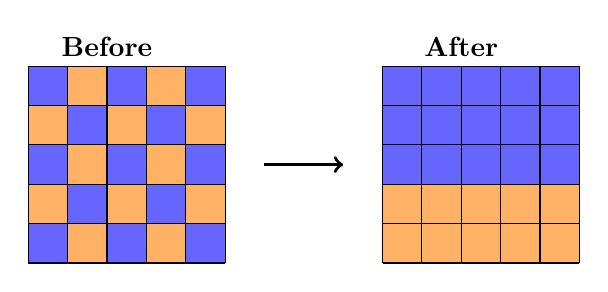
\begin{tikzpicture}[scale=0.5]
    % Before grid (checkerboard pattern)
    \node at (2, 5.5) {\textbf{Before}};
    % Row 0
    \fill[blue!60] (0,0) rectangle (1,1); \fill[orange!60] (1,0) rectangle (2,1);
    \fill[blue!60] (2,0) rectangle (3,1); \fill[orange!60] (3,0) rectangle (4,1);
    \fill[blue!60] (4,0) rectangle (5,1);
    % Row 1
    \fill[orange!60] (0,1) rectangle (1,2); \fill[blue!60] (1,1) rectangle (2,2);
    \fill[orange!60] (2,1) rectangle (3,2); \fill[blue!60] (3,1) rectangle (4,2);
    \fill[orange!60] (4,1) rectangle (5,2);
    % Row 2
    \fill[blue!60] (0,2) rectangle (1,3); \fill[orange!60] (1,2) rectangle (2,3);
    \fill[blue!60] (2,2) rectangle (3,3); \fill[orange!60] (3,2) rectangle (4,3);
    \fill[blue!60] (4,2) rectangle (5,3);
    % Row 3
    \fill[orange!60] (0,3) rectangle (1,4); \fill[blue!60] (1,3) rectangle (2,4);
    \fill[orange!60] (2,3) rectangle (3,4); \fill[blue!60] (3,3) rectangle (4,4);
    \fill[orange!60] (4,3) rectangle (5,4);
    % Row 4
    \fill[blue!60] (0,4) rectangle (1,5); \fill[orange!60] (1,4) rectangle (2,5);
    \fill[blue!60] (2,4) rectangle (3,5); \fill[orange!60] (3,4) rectangle (4,5);
    \fill[blue!60] (4,4) rectangle (5,5);
    % Grid lines
    \draw (0,0) grid (5,5);
    
    % Arrow
    \draw[->, very thick] (6, 2.5) -- (8, 2.5);
    
    % After grid (segregated)
    \node at (11, 5.5) {\textbf{After}};
    % Bottom rows (orange)
    \fill[orange!60] (9,0) rectangle (14,2);
    % Top rows (blue)
    \fill[blue!60] (9,2) rectangle (14,5);
    % Grid lines
    \draw (9,0) grid (14,5);
\end{tikzpicture}
\captionof{figure}{Schelling's Model: emergent segregation.}
\end{center}
\end{itemize}

\section{Normal Form Games}

\subsection{Definitions}
\begin{definition}
A \textbf{normal form game} is a triplet $(N, (X_i)_{i \in N}, (u_i)_{i \in N})$ where:
\begin{itemize}
    \item $N$ is the set of players.
    \item $X_i$ is the set of actions for player $i \in N$.
    \item $u_i: X \rightarrow \mathbb{R}$ is the payoff function.
    \item $X = \prod_{i \in N} X_i$ represents the set of \textbf{action profiles}. A profile is a list $x = (x_1, x_2, \dots, x_n)$ containing an action for each player.
\end{itemize}
\end{definition}

\subsection{Famous Examples}

\begin{enumerate}
    \item \textbf{Coordination Game:}
    \begin{center}
    \begin{tabular}{c|c|c}
     & A & B \\ \hline
    A & (1, 1) & (0, 0) \\ \hline
    B & (0, 0) & (2, 2)
    \end{tabular}
    \end{center}

    \item \textbf{Chicken Game / Hawk-Dove:}
    \begin{center}
    \begin{tabular}{c|c|c}
     & Swerve & Straight \\ \hline
    Swerve & (0, 0) & (-1, 1) \\ \hline
    Straight & (1, -1) & (-10, -10)
    \end{tabular}
    \end{center}

    \item \textbf{Matching Pennies:}
    \begin{center}
    \begin{tabular}{c|c|c}
     & Heads & Tails \\ \hline
    Heads & (1, -1) & (-1, 1) \\ \hline
    Tails & (-1, 1) & (1, -1)
    \end{tabular}
    \end{center}

    \item \textbf{Prisoner's Dilemma:}
    \begin{center}
    \begin{tabular}{c|c|c}
     & Don't Confess & Confess \\ \hline
    Don't Confess & (-1, -1) & (-10, 0) \\ \hline
    Confess & (0, -10) & (-5, -5)
    \end{tabular}
    \end{center}

    \item \textbf{Guess two-thirds of the average:}
    This game illustrates that your optimal strategy depends on your ability to guess the rationality level of other players.
\end{enumerate}

\subsection{Examples of Continuous Games}

\paragraph{First-Price Auction}
$N = \{1, 2\}$, $X_1 = X_2 = [0, +\infty[$. Values $v_1 = 1M, v_2 = 1.1M$.
$$u_i(x_i, x_j) = \begin{cases} v_i - x_i & \text{if } x_i > x_j \\ \frac{v_i - x_i}{2} & \text{if } x_i = x_j \\ 0 & \text{otherwise} \end{cases}$$

\begin{center}
\begin{tikzpicture}[scale=0.8]
    \draw[->] (0,0) -- (5,0) node[right] {$x_1$};
    \draw[->] (0,-0.5) -- (0,3) node[above] {$u_1$};
    % u_1 = 0 for x_1 < x_2
    \draw[thick, blue] (0,0) -- (2,0);
    % Discontinuity at x_1 = x_2
    \fill[blue] (2,0) circle (2pt);
    \draw[blue, dashed] (2,0) -- (2,1.5);
    \fill[white] (2,1.5) circle (2pt);
    \draw[blue] (2,1.5) circle (2pt);
    % u_1 = v_1 - x_1 for x_1 > x_2
    \draw[thick, blue] (2,1.5) -- (4,0.5);
    % Labels
    \node[below] at (2,0) {$x_2$};
    \node[left] at (0,1.5) {$v_1 - x_2$};
    \draw[dashed, gray] (0,1.5) -- (2,1.5);
\end{tikzpicture}
\captionof{figure}{Payoff $u_1(x_1)$ for fixed $x_2$: discontinuity at $x_1 = x_2$.}
\end{center}
\begin{figureexplanation}
This graph illustrates the payoff discontinuity in a first-price auction.
\begin{itemize}
    \item If the player bids $x_1 < x_2$, they lose and get 0.
    \item If they bid $x_1 = x_2$, they split the payoff 50\% (white dot/circle).
    \item If they bid $x_1 > x_2$ (even by a tiny amount), they win the whole market (abrupt jump in payoff).
\end{itemize}
This discontinuity prevents the direct application of Nash's theorem (which requires continuous payoff functions).
\end{figureexplanation}

\paragraph{Second-Price Auction (Vickrey)}
Two players $i=1,2$ with valuations $v_i$. They submit bids $x_i \ge 0$. The winner pays the loser's bid.
\[
u_1(x_1, x_2) = 
\begin{cases} 
v_1 - x_2 & \text{if } x_1 > x_2 \\
\frac{v_1 - x_2}{2} & \text{if } x_1 = x_2 \\
0 & \text{if } x_1 < x_2
\end{cases}
\]

\section{Exercises}

\begin{exemple}[All pay auction]
All bidders pay their bid, whether they win the object or not. The highest bidder wins the object.
\begin{itemize}
    \item \textbf{Mechanism:} Each player submits a bid $x_i \ge 0$.
    \item \textbf{Payoff function:} For player $i$, with valuation $v_i$:
    \[ u_i(x_i, x_{-i}) = \begin{cases} v_i - x_i & \text{if } x_i > x_j \quad \forall j \neq i \\ -x_i & \text{if } x_i < \max(x_{-i}) \end{cases} \]
    (In case of a tie for the highest bid, the payoff might be shared).
\end{itemize}
\end{exemple}

\begin{exemple}[Ice-cream sellers (Hotelling)]
\textbf{Task:} Two sellers position themselves on the interval $[0, 1]$. Customers are uniformly distributed and go to the nearest seller.
\begin{enumerate}
    \item Formally write down the payoff functions.
    \item Plot $u_1(x_1, x_2)$ for a fixed value $x_2 < 1$.
\end{enumerate}

\paragraph{Solution:}
\begin{enumerate}
    \item Customers choose the nearest seller. The "indifferent" customer is located at the midpoint between the two sellers, i.e., at $m = \frac{x_1 + x_2}{2}$.
   If $x_1 < x_2$, Seller 1 captures all customers in $[0, m]$. Their payoff (market share) is:
   $$u_1(x_1, x_2) = \frac{x_1 + x_2}{2}$$
   If $x_1 > x_2$, Seller 1 captures customers in $[m, 1]$. Their payoff is:
   $$u_1(x_1, x_2) = 1 - \frac{x_1 + x_2}{2}$$
   If $x_1 = x_2$, they share the market: $u_1 = 1/2$.

    \item For a fixed $x_2$ (say $x_2 = 0.7$), here is the shape of $u_1(x_1)$:
\begin{center}
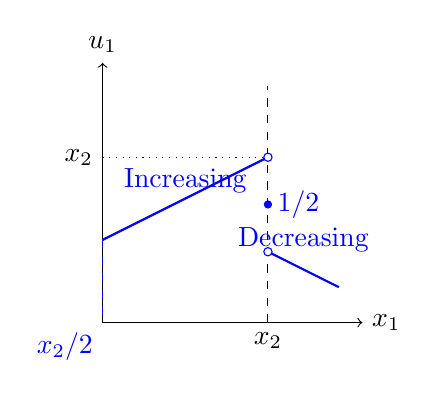
\begin{tikzpicture}[scale=3]
    \draw[->] (0,0) -- (1.1,0) node[right] {$x_1$};
    \draw[->] (0,0) -- (0,1.1) node[above] {$u_1$};
    \node[below] at (0.7,0) {$x_2$};
    \draw[dashed] (0.7,0) -- (0.7,1);
    
    % First part: increasing
    \draw[thick, blue] (0,0.35) -- (0.7,0.7); % Starts at 0.7/2 = 0.35, ends at 1.4/2 = 0.7
    \draw[dashed, blue] (0,0.35) -- (0,0) node[below left] {$x_2/2$};
    
    % Point at x2
    \fill[white] (0.7,0.7) circle (0.5pt);
    \draw[blue] (0.7,0.7) circle (0.5pt);
    
    \fill[blue] (0.7,0.5) circle (0.5pt) node[right] {1/2}; % At x1=x2
    
    % Second part: decreasing
    \draw[thick, blue] (0.7,0.3) -- (1,0.15); 
    
    \fill[white] (0.7,0.3) circle (0.5pt);
    \draw[blue] (0.7,0.3) circle (0.5pt);
    
    \draw[dotted] (0,0.7) -- (0.7,0.7) node[left] at (0,0.7) {$x_2$}; 
    
    \node[blue] at (0.35, 0.6) {Increasing};
    \node[blue] at (0.85, 0.35) {Decreasing};
\end{tikzpicture}
\end{center}
The maximum is reached just "before" $x_2$ (to capture the entire left market). At equilibrium, both position themselves at the center ($1/2$).
\end{enumerate}
\end{exemple}
